\chapter{Introduction}

\section{Introduction}
Fusion techniques are very common in our nature. Animals sense the environment by eyes, ears etc. We, Humans, also have the ability to collect data about the environment model by five body senses. We can enrich the perceived environment model by combining all senses data \cite{Wilfried2002}. Like nature, science also adopt the fusion concept and successfully applied in its many fields. For example, self driving car needs to sense the environment by the sensors and sensor fusion helps to perceive the environment model more correctly. This paper tries to explain the basic concept of Sensor Fusion and also explains some of the applications of this concept.

\section{What is Sensor Fusion?}
The term \emph{Sensor Fusion} means fusing multiple sensor data to make a rich environment model. One sensor data may not cover all the information or in some cases one sensor may produces incomplete information. Fusion of multiple sensors data improves the quality of the data and produce more reliable environment model. According to \cite{Hall:2004:MTM:1204261} the term \emph{multisensor data fusion} defined as,
\theoremstyle{definition}
\begin{definition}{Multisensor data fusion}
is the technology concerned with the combination of how to combine data from multiple (and possible diverse) sensors in order to make inferences about a physical event, activity, or situation.
\end{definition}
On the other hand, the more formal definition of Sensor Fusion is defined in \cite{Wilfried2002} as,
\theoremstyle{definition}
\begin{definition}{Sensor Fusion}
is the combining of sensory data or data derived from sensory data such that the resulting information is in some sense better than would be possible when these sources were used individually.
\end{definition}
There is a confusion about \emph{multisensor integration} and \emph{sensor fusion}. In multisensor integration, data is received from multiple sensor but it is send to the control application directly without fusion. In sensor fusion, data also comes from multiple sensor but the control application get the fused data which is only one single representation of environment model and the control application gets only one data.

\section{Motivation for Sensor Fusion}
The following scenarios are very common which may fails physical sensor measurement\cite{Wilfried2002}:
\begin{description}
    \item[Sensor Element Broken:] A sensor is composed with some small elements. If one of the elements are broken, it would give incomplete results. Incomplete results would be produced for some other reasons, such as calibration issues,hardware malfunctions, uncertain detection and asynchronous scans, even from scene perturbations, like occlusions, weather issues and object shifting.
    \item[Only Covering Restricted Region:] An individual sensor has the capability of covering a limited range. For example, a camera sensor facing to the front side of a car could not cover the back side of the car.
    \item[Processing Time:] Some sensors are limited to processing power so that they need some time to capture and transmit the data. As a result, the frequency of measurement is also decreased. For example, a very complex camera sensor may sends the captured image of a pedestrian crossing the road after one or two seconds which is very risky for self driving car.
    \item[Uncertainty:] The single sensor measurement could be uncertain. For example, a distance sensor facing to the front of a car may capture the correct distance from a object or may be the sensor beam misses the object and giving the wrong distance. Actually, uncertainty occurs for missing functionality (e.g., occlusions) and also when sensor can not measure all relevant attributes of precept, or when the observation is ambiguous\cite{Wilfried2002}. Because of having coverage of limited region, a single sensor may produce uncirtain result\cite{Wilfried2002}.
\end{description}
Sensor Fusion could solves problems given above. The following advantages can be expected from sensor fusion over a single sensor\cite{Wilfried2002}:
\begin{description}
    \item[Robustness and reliability:] Depending on multiple sensor increase the redundancy of data and even if one of the sensors are broken, we expect accurate data.
    \item[Extended Coverage:] By multiple sensor, the environment can be observed from different faces and different angle.
    \item[Processing Parallel:] One sensor can take some time to process and other sensor can capturing and again when one finish processing start capturing and other stat processing.
    \item[Reduce Uncertainty:] Getting same data from multiple sensor reduce the uncertainty. For example, one sensor may miss the object but other may capture.
    \item[Prevent Interruption:] Using different types of sensors for same purpose can prevent interruption. For example, a self driving car is driving while raining and the camera sensor could not see the actual objects in-front of it because of rain drops. In this case, parallel performing an ultrasonic sensor can still measure the objects.
    \item[Improved Quality:] Getting same data from multiple source increasing the quality of the data.
\end{description}
One of the interesting advantage of sensor fusion is the possibility to reduce system complexity\cite{Wilfried2002}. It is possible to consider the sensor fusion component as a separate system and the main control system could communicate with it via defined interface. To do so we can modify the fusion subsystem without touching the main system\cite{Wilfried2002}.

\section{Categories of Sensor Fusion}
Sensor Fusion is categorized by different applications in aspects. In the following parts, the categories are described.

\subsection{Three-Level Categorization}
According to level of data the fusion process can be categorized by following criteria:
\begin{description}
    \item[Low-level fusion] is also known as \emph{raw data fusion} refers to fusion of raw data from multiple sensor and combine them to produce new data which is more reliable and understandable than the raw data.
    \item[Intermediate-level fusion] is also knows as \emph{feature level fusion} refers to collecting a bunch of features and keep the features into a feature map which can be used by AI applications like segmentation and detection of objects. For example, keeping features like edges, corners, lines are useful for pedestrians detection.
    \item[High-level fusion] is also known as \emph{decision fusion} refers to making decisions from several sensors. For example, voting, fuzzy-logic and statistical methods.\cite{Wilfried2002}.
\end{description}

\subsection{Categorization Based on Input/Output}
Dasarathy extend the three-Level categorization based on input/output\cite{Wilfried2002}. Actually if the input output are considered then the input of one level comes from another level. For example, the input of feature extraction comes from raw data and the raw data produce selection of some features. So, the levels are not same anymore.  In Figure \ref{fig:InputoutputCat}, the relation between three-Level categorization and input/output is shown.
\begin{figure}
  \centering
  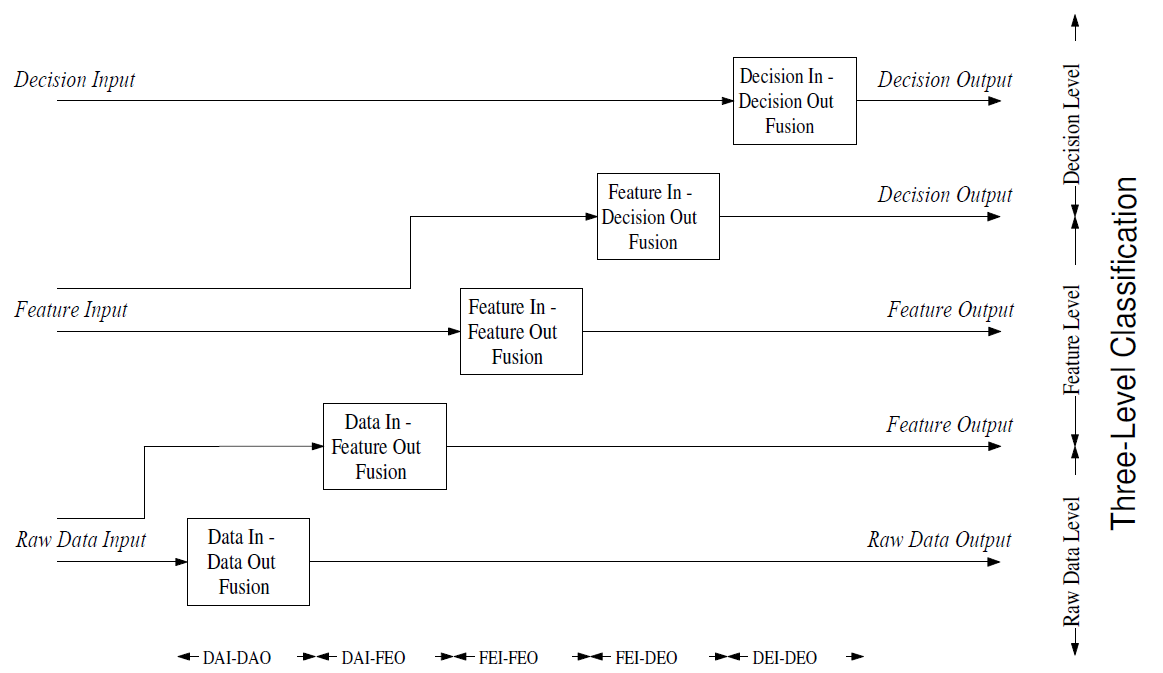
\includegraphics[width=1.1\textwidth]{src/pic/InputoutputCat.png}
  \caption{Fusion Categorization by input/output}
  \label{fig:InputoutputCat}
\end{figure}

\subsection{Categorization Based on Sensor Configuration}
Sensor fusion may be in different configuration types. According to various configuration, sensor fusion can be categorized into three sections\cite{Wilfried2002}:
\begin{description}
    \item[Complementary:] A configuration is considered as a complementary configuration when the sensors participating in sensor fusion are not directly dependent on each other, but it would be a case where inputs of the sensors are mixed to produce complete result. This configuration solves on of the common problem of single sensor system which is incompleteness of sensor data.
    \item[Competitive:] Competitive configuration can be achieved by keeping multiple sensors for observing same object or view which are independent from each other. This configuration ensure high redundancy of data and that is why it is also called \emph{redundant configuration}\cite{Wilfried2002}.
    \item[Cooperative:] A cooperative mechanism is the intelligent one in a sense that in this configuration the inputs from separate sensors are combined to produce a information which is not available in the single sensor inputs. An example for a cooperative sensor configuration is stereoscopic vision - by combining two-dimensional images from two cameras at slightly different viewpoints a three-dimensional image of the observed scene is derived\cite{Wilfried2002}.
\end{description}

There could be more categories exists but commonly used sensors are categorized like above. 

\section{Commonly used Sensor Fusion Models/Applications}

\subsection{Evidential Framework}
The Evidential framework is a generalization of the Bayesian framework of subjective probability\cite{Chavez_Garcia_2016}. Evidential theory (ET) is applicable to the problems which are ambiguous and unpredictable for finding solutions. We can apply it on uncertain problems to have a belief based on available proofs. There are two major concepts, mass function and belief function to perform uncertainty reasoning\cite{Bell_4028391}.\\
Assume, $\Omega$ is a set of hypotheses over a hypothesis space. A function $m:2^\Omega \rightarrow[0, 1]$ is called mass function which is defined as follows\cite{Bell_4028391}:
$$M1. m(\emptyset)=0$$
$$M2.\sum_{x \subseteq \Omega} m(X) = 1$$
where, $\emptyset$ is an empty set, $X$ is a variable and the assigned uncertainties are called $m-$values\cite{srivastava2011introduction}. For the variable $X$, we can have $m(x) \geq 0$, $m(\neg x) \geq 0$, and $m(\{x,\neg x\}) \geq 0$, such that $m(x) + m(\neg x) + m(\{x,\neg x\}) = 1$\cite{srivastava2011introduction}. We can have $m-$values for all the subsets of single element, double element, triple element and so on over the a hypothesis space and this hypothesis space contains all probable values of variable $X$. For example, a proof $Pr_{1}$ is $m_{1}(x)=0.8$, $m_{1}(\neg x)=0.15$ and $m_{1}(\{x,\neg x\}) = 0.05$. It means $80\%$ agree that $X$ is $\mathbb true$, $15\%$ agree that $X$ is $\mathbb false$ and $5\%$ are not sure reflecting ignorance.\\
Another function $bel:2^\Omega \rightarrow[0, 1]$ is called belief function which is defined as follows\cite{srivastava2011introduction}:
$$bel(O) = \sum_{C \subseteq O} m(C)$$
where, $O$ is a set of elements which is the summation of all $m-$values of that set of elements denoted by $C$. As like probability theory it is not needed  to be $1$ the summation of belief in $O$ and belief in $\neg O$ which is actually less or equal to $1$, i.e., $bel(O) + bel(\neg O)\leq 1$\cite{srivastava2011introduction}. Zero belief, i.e., $bel(x) = 0$, and $bel(\neg x) = 0$ indicates the lack of proofs, also in other other word it indicates ignorance. For example, again consider the previous example $Pr_{1}$. In this case, $bel_{1}(x) = m_{1}(x) = 0.8$, $bel_{1}(\neg x) = m_{1}(\neg x) = 0.15$ and $bel_{1}(\{x, \neg x\}) = m_{1}(x) + m_{1}(\neg x) + m_{1}({x, \neg x}) = 0.8+0.15+0.5 = 1$.\\
The fundamental operation of evidential reasoning is the orthogonal sum of evidential function (mass and belief function), which is known as Dempster's rule for combining proofs\cite{Bell_4028391}. The Dempster's rule to combine $m-$values can be written as (Shafer 1976) follows\cite{srivastava2011introduction}:
 $$m(O \neq \emptyset) = \frac{1}{k}  \sum_{O=C_{1} \cap C_{2}} m_{1}(C_{1})m_{2}(C_{2})$$
where, $K$ is the renormalization constant and 
$$K = \sum_{C_{1} \cap C_{2} \neq \emptyset} m_{1}(C_{1})m_{2}(C_{2}) = 1-\overbrace{ \sum_{C_{1} \cap C_{2} = \emptyset} m_{1}(C_{1})m_{2}(C_{2})}^{CV}$$
$CV$ in $K$ indicates the conflict value which is distributed among all the elements of the frame of discernment\cite{Chavez_Garcia_2016}.\\
Generally, ET considers three situations, $\mathbb true$, $\mathbb false$ and not sure (ignorance) by which it can find solutions for ambiguous and unpredictable problems more powerfully. For example, an online shop's admin wants to know the degree of satisfaction for a delivered product $A$ from the customers. The answer from customer $C_{1}$ is $80\%$ satisfied, $15\%$ unsatisfied, $5\%$ not sure. Answer from another customer $C_{2}$ is $60\%$ satisfied, $20\%$ unsatisfied, $30\%$ not sure. Assume, a hypothesis space is, $\Omega = \{S, U\}$ where $S$ and $U$ stand for satisfiability and unsatisfiability respectively. So, we have two set of proofs for $C_{1}$ and $C_{2}$. According to ET, the combination of two proofs can be represented in Table \ref{table:customer_surv} \cite{Bell_4028391}.
\begin{table}[]
\centering
\caption{Combination of two customer surveys}
\label{table:customer_surv}
\begin{tabular}{|l|l|l|l|}
\hline
 $m^{\prime}=C_{1}\oplus C_{2}$&  $m_{1}(S)=0.8$ & $m_{1}(U)=0.15$ & $m_{1}(\{S, U\})=0.5$ \\ \hline
 $m_{2}(S)=0.6$& $0.8x0.6=0.48$ & $\emptyset$ & $0.6x0.05=0.03$ \\ \hline
 $m_{1}(U)=0.2$& $\emptyset$ & $0.2x0.15=0.03$ & $0.2x0.05=0.01$ \\ \hline
 $m_{1}(\{S, U\})=0.3$& $0.3x0.8=0.24$ & $0.3x0.15=0.045$ & $0.3x0.05=0.015$ \\ \hline
\end{tabular}
\end{table}
By applying Dempster's rule, we get as follows:
$$K = \sum_{C_{1} \cap C_{2} \neq \emptyset} m_{1}(C_{1})m_{2}(C_{2}) = 1- \sum_{C_{1} \cap C_{2} = \emptyset} m_{1}(C_{1})m_{2}(C_{2})$$
$$=0.48 + 0.03 + 0.03 + 0.01 + 0.24 + 0.045 + 0.015 = 0.85$$
$$m^{\prime}(S)=(\frac{1}{0.85})(0.48 + 0.03 + 0.24) = 0.882$$
$$m^{\prime}(U)=(\frac{1}{0.85})(0.03+0.01+0.045) = 0.1$$
$$m^{\prime}(\{S, U\})=(\frac{1}{0.85})(0.015) = 0.017$$
So, the combination result is $88.2\%$ satisfied, $10\%$ unsatisfied and $1.7\%$ undecided. Authors has used this evidential approach based on mass distributions over the set of different class hypotheses\cite{Chavez_Garcia_2016}.

\subsection{Kalman Filter}
The Kalman Filter(KF) is a linear mathematical model which uses a recursive algorithm for filtering signals by measuring a respectable amount of statistical and systematical errors\cite{Wilfried2002}. It was developed by Kalman and Bucy in 1960\cite{Wilfried2002}.KF generates a estimation of the true and measured values\cite{aich2010study}. First, it predicts a value. Then it measures the ambiguity of previous value. Finally, it performs an weighted average of both the predicted and measured values\cite{aich2010study}.
The more the weight is, the less the ambiguity is. The output of a KF is the estimation which is closer to true values. This is the basic operation of a KF.

A standard KF model is explained by two linear equations\cite{Wilfried2002}. The first equation measures the state of a system at time $k$ which is governed by the linear stochastic difference equation\cite{aich2010study}:
$$\vec{x}_{k} = A \cdot \vec{x}_{k-1} + B \cdot \vec{u}_{k-1} + w_{k-1}$$
\begin{table}[!htbp]
\centering
\label{my-label}
\begin{tabular}{llll}
where, & $\vec{x}_{k-1}$     & = & a vector representing the state at time $k-1$                                                                                                                                         \\
       & $A$       & = & non singular state transition matrix                                                                                                                                                  \\
       & $\vec{u}_{k-1}$     & = & a vector representing the input of the system at time $k-1$                                                                                                                           \\
       & $B$       & = & The relation between $\vec{x}_{k-1}$ and $\vec{u}_{k-1}$                                                                                                                                                  \\
       & $w_{k-1}$ & = & a random variable representing the process noise, \\
       &        & & modelled as white noise $\sim N(0; Q)$, where $Q$ is the covariance matrix
\end{tabular}
\end{table}\\
with a measurement which is the second equation\cite{aich2010study}:
$$\vec{z_{k}} = H \cdot \vec{x_{k}} + v_{k} $$
\begin{table}[!htbp]
\centering
\label{my-label}
\begin{tabular}{llll}
where, & $\vec{z_{k}}$     & = & a vector representing the sensor observation at time $k$                                                                                                                                         \\
       & $H$       & = & a matrix relates the measurements to the internal state                                                                                                                                            \\
       & $v_{k}$ & = & a random variable representing the measurement noise, \\
       &        & & also modelled as white noise $\sim N(0; Q)$, where $R$ is the covariance matrix
\end{tabular}
\end{table}

\subsubsection{Kalman Filtering Algorithm}
To start a KF, user has to give an estimation $\vec{x_{0}}$ and an estimate of its covariance $P_{0|0}$ i.e., inaccurate start value. After initialization user can traverse the Kalman Filtering Algorithm. It has following steps\cite{Wilfried2002}:
\begin{enumerate}
  \item  Compute a predicted priori state estimation of state $\vec{x}$ at time $k$ by using given observations up to $k-1$.
  $$\vec{x}_{k|k-1} = A\cdot \vec{x}_{k-1|k-1} + B\cdot \vec{u}_{k-1}$$
  \item Compute predicted error covariance matrix at time $k$.
  $$P_{k|k-1} = A \cdot P_{k-1|k-1} \cdot A|{T} + Q$$
  \item Compute Kalman gain.
  $$K_{k} = \frac{P_{k|k-1} \cdot C^{T}}{C \cdot P_{k|k-1} \cdot C^{T} + R}$$
  \item Update the estimation by a measurement $z_{k}$.
  $$\vec{x}_{k|k} = \vec{x}_{k|k-1} + k_{k} \cdot (z_{k} - C \cdot \vec{x}_{k|k-1})$$
  \item Update error covariance matrix.
  $$P_{k|k} = (I - k_{k} \cdot C) P_{k+1|k} (I - k_{k} \cdot C)^{T} + k_{k} \cdot R \cdot k^{T}_{k}$$
  where, $I$ is the identity matrix.
\end{enumerate}

After performing these 5 steps the iteration restarts again from step 1, but with $k:=k+1$.\\
So, we can say that The equations containing in the steps of above algorithm can be divided into two groups: time update equations (equation 1 and 2) and measurement update equations(equation 3-5)\cite{bishop2001introduction}. Also the final estimation algorithm looks like  a predictor-corrector algorithm as shown in Figure \ref{fig:kalman_cycle}.

\begin{figure}
  \centering
  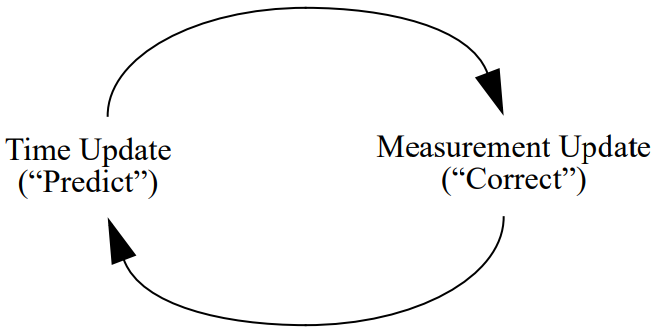
\includegraphics[width=.4\textwidth]{src/pic/kalman_cycle.png}
  \caption{Kalman Filter Cycle \cite{bishop2001introduction}}
  \label{fig:kalman_cycle}
\end{figure}

\begin{figure}
  \centering
  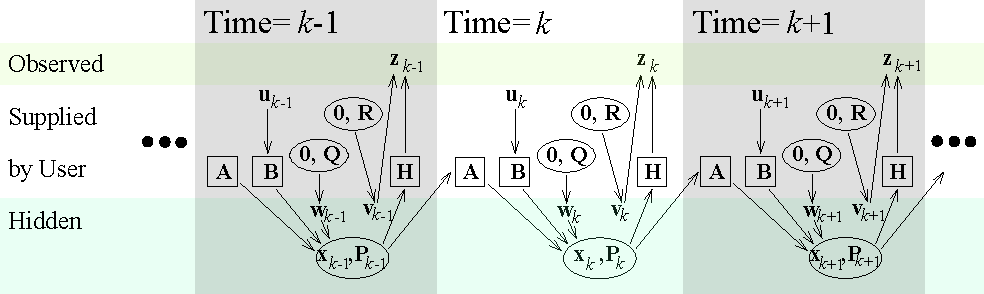
\includegraphics[width=1\textwidth]{src/pic/Kalman_filter_model_2.pdf}
  \caption{Underlying Model of the Kalman Filter \cite{aich2010study}}
  \label{fig:Kalman_filter_model_2}
\end{figure}

\subsubsection{Underlying Dynamic System Model}
KF is based on linear and non-linear dynamical systems discretized in the time domain\cite{bishop2001introduction}. As shown in Figure \ref{fig:Kalman_filter_model_2}, each state represents a real vector and a sequence of noisy observations are the inputs of internal states. The system is modeled according to the state space representation of the KF specifying the matrices i.e., the state transition model ($A$), the observation model ($H$), the covariance of the process noise ($Q$), the covariance of the measurement noise ($R$), and sometimes the control-input model ($B$) for each time-step $k$.\\
There are lot of dynamic systems which do not support KF as it is a linear model\cite{aich2010study}. To deal with these type of dynamic systems Extended KF and Unscented KF are used which are the extended version KF\cite{aich2010study}.

\subsection{Extended Kalman Filter}
The extended Kalman filter (EKF) is the nonlinear version of the Kalman filter which linearizes about the current mean and covariance \cite{aich2010study}. In the EKF, the transition state ($\vec{x}_{k}$) and observation state ($\vec{z}_{k}$) space models may not be linear functions of the state as like KF but might be many non-linear functions \cite{aich2010study}.\\
Like KF, an EKF model is also explained by two linear equations, but The first equation measures the state of a system at time $k$ which is now governed by the non-linear stochastic difference equation\cite{aich2010study}:
$$\vec{x}_{k} = f( \vec{x}_{k-1}, \vec{u}_{k-1}) + w_{k-1}$$
with a measurement which is the second equation\cite{aich2010study}:
$$\vec{z_{k}} = h( \vec{x_{k}}) + v_{k} $$
where, the random variables $w_{k}$ and $v_{k}$ again represent the process and measurement noise as like in KF. These random variables are assumed to be zero with covariance $Q_{k}$ and $R_{k}$ respectively\cite{aich2010study}. The non-linear functions $f$ relates the state at time step $k-1$ to the state at step $k$ and $h$ relates
the state $\vec{x}_{k}$ to the measurement $\vec{z}_{k}$\cite{bishop2001introduction}. At each time step with the help of current prediction the Jacobian (a matrix of partial derivatives) is calculated, because  $f$ and $h$ cannot
be used to the covariance directly.It is used in the EKF equations which linearizes the non-linear functions\cite{aich2010study}.
\subsubsection{Extended Kalman Filtering Algorithm}
The initialization part is exactly like the Kalman Filtering Algorithm. It has the following steps\cite{aich2010study}:
\begin{enumerate}
  \item  Compute a predicted priori state.
  $$\vec{x}_{k|k-1} = f( \vec{x}_{k-1|k-1} + \vec{u}_{k-1})$$
  \item Compute predicted error covariance matrix at time $k$.
  $$P_{k|k-1} = F_{k}P_{k-1|k-1} F{_{k}}^T + Q$$
  where, $F_{k-1} = \frac{\partial f}{\partial x} |_{\vec{x}_{k-1|k-1},\vec{u}_{k-1}}$ (Jacobian).
  \item Compute Kalman gain.
  $$K_{k} = P_{k|k-1}H_{k}S{_{k}}^{-1}$$
  where, $H_{k} = \frac{\partial h}{\partial x} |_{\vec{x}_{k|k-1}}$ (Jacobian) and $S_{k} = H_{k}P_{k|k-1}H{_{k}}^T + R$ (innovation or residual covariance).
  \item Update the estimation by a measurement $z_{k}$.
  $$\vec{x}_{k|k} = \vec{x}_{k|k-1} + K_{k}\tilde y_{k}$$
  where $\tilde y_{k}=z_{k}-h(\vec{x}_{k|k-1})$ (innovation or measurement residual).
  \item Update error covariance matrix.
  $$P_{k|k} = (I - k_{k}H_{k})P_{k|k-1}$$
  where, $I$ is the identity matrix.
\end{enumerate}
After performing these 5 steps the iteration restarts again from step 1, but with $k:=k+1$.
So, Extended Kalman Filtering Algorithm is also the same as the linear discrete KF as shown in Figure \ref{fig:kalman_cycle}\cite{bishop2001introduction}.



